\documentstyle[11pt,epsfig,fancybox,semcolor,semlayer,doublespace,landscape]
{seminar}
\input clp_utils

\newcommand{\talktitle}[0]{Rich's Question}
\newcommand{\fmttitle}[0]{}
\newcommand{\conftitle}[0]{A Exam}
\newcommand{\myname}[0]{Jim Pivarski}
\newcommand{\affila}[0]{Cornell University}
\newcommand{\talkdate}[0]{October 3, 2002}

\pagestyle{conference}   % From clp_utils.tex

% slide magnification
\slidesmag 1

%%%%%%%%%%%%%%%%%%%%%%%%%%%%%%%%%%%%%%%%%%%%%%%%%%%%%%%%%%%%%%%%%%%%%%%%%%%
% Start document
\begin{document}

% Set page size
\slideheight 7.0in
\slidewidth 8.8in 

% Set array stretch
\renewcommand{\arraystretch}{0.3}
\renewcommand{\slidetopmargin}{0.4in}
\renewcommand{\slidebottommargin}{0.9in}


%%%%%%%%%%%%%%%%%%%%%%%%%%%%%%%%%%%%%%%%%%%%%%%%%%%%%%%%%%%%%%%%%%%%%%%%%%%

% %%%%%%%%%%%%%%%%%%%%%%%%%%%%%%%%%%%%%%%%%%%%%%%%%%%%%%%%%%%%%%%%%%%%%%%%%%%

% \begin{slide*}

% \slideframe{}
% \slideframe*[\dkblue]{Oval}
% \huge
% \heading{Outline}
% \vspace{1 cm}

% \begin{center}
% \begin{minipage}[t]{12 cm}
% \begin{itemize}
% \LARGE \item {\huge Motivation: verify lattice QCD!}
% \LARGE \item {\huge 2 out of 3 Resonances Scanned}
% \LARGE \item {\huge Energy Calibration Systematics}
% \LARGE \item {\huge Other Systematics / Work to be Done}
% \end{itemize}
% \end{minipage}
% \end{center}

% \end{slide*}
 
%%%%%%%%%%%%%%%%%%%%%%%%%%%%%%%%%%%%%%%%%%%%%%%%%%%%%%%%%%%%%%%%%%%%%%%%%%%

\begin{slide*}

\slideframe{}
\slideframe*[\dkblue]{Oval}

\begin{center}
  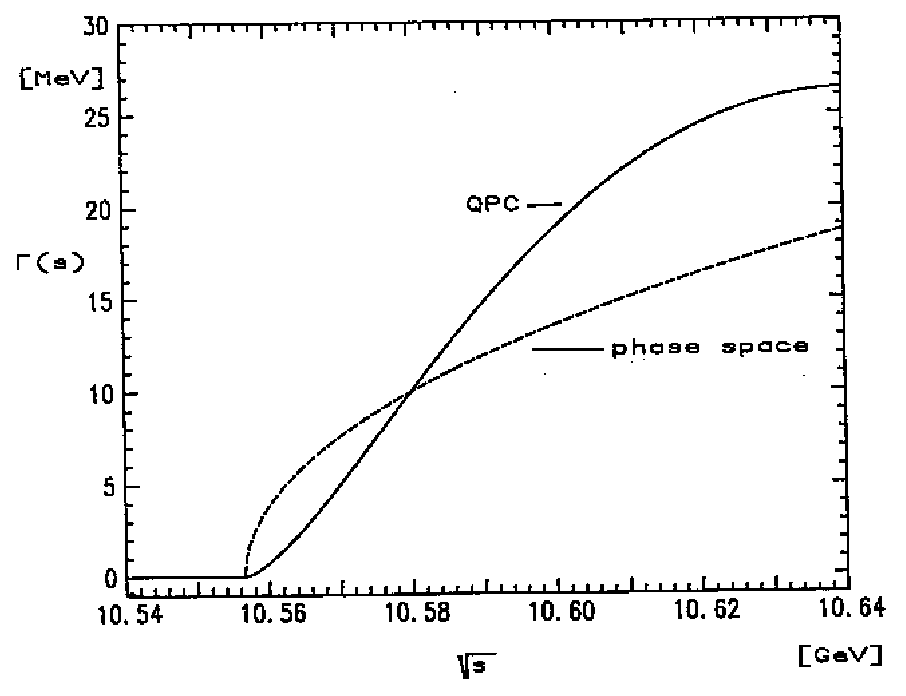
\epsfig{file=gamma_from_models.eps, width=0.5\textheight, angle=-90} \\
  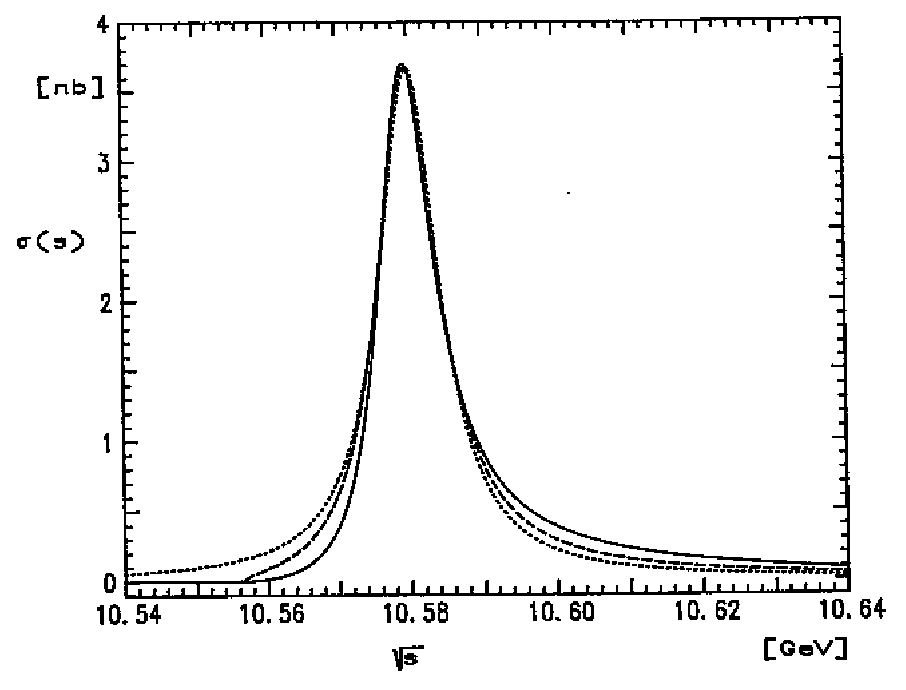
\epsfig{file=peak_from_models.eps, width=0.5\textheight, angle=-90}
\end{center}

\end{slide*}

%%%%%%%%%%%%%%%%%%%%%%%%%%%%%%%%%%%%%%%%%%%%%%%%%%%%%%%%%%%%%%%%%%%%%%%%%%%

\begin{slide*}

\slideframe{}
\slideframe*[\dkblue]{Oval}

\begin{center}
  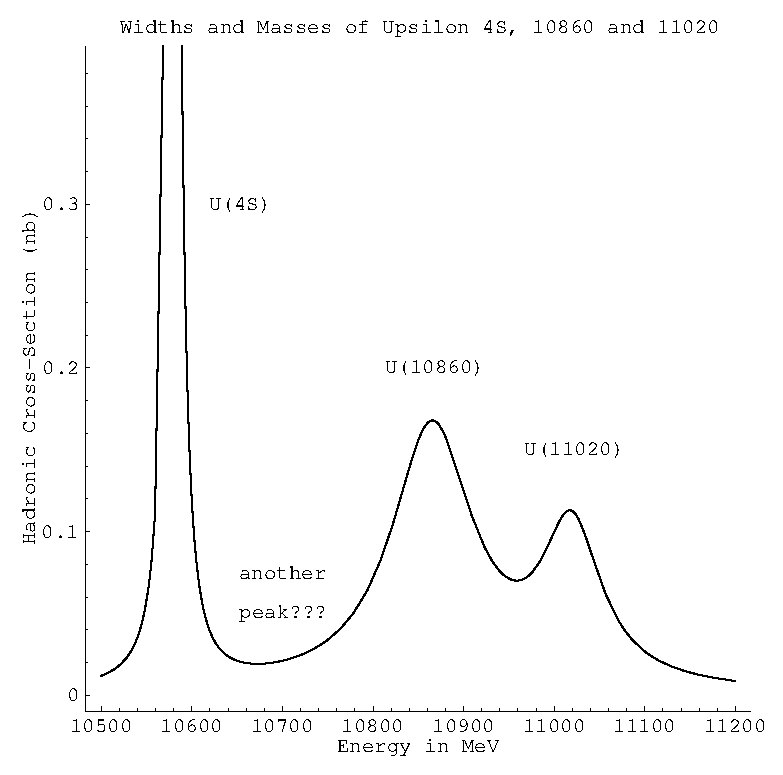
\epsfig{file=theopeaks.eps, width=0.5\textheight, angle=-90} \\
  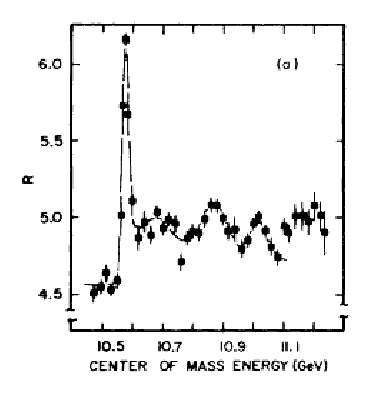
\epsfig{file=exptpeaks.eps, width=0.5\textheight, angle=-90}
\end{center}

\end{slide*}

%%%%%%%%%%%%%%%%%%%%%%%%%%%%%%%%%%%%%%%%%%%%%%%%%%%%%%%%%%%%%%%%%%%%%%%%%%%

\begin{slide*}

\slideframe{}
\slideframe*[\dkblue]{Oval}

\begin{center}
  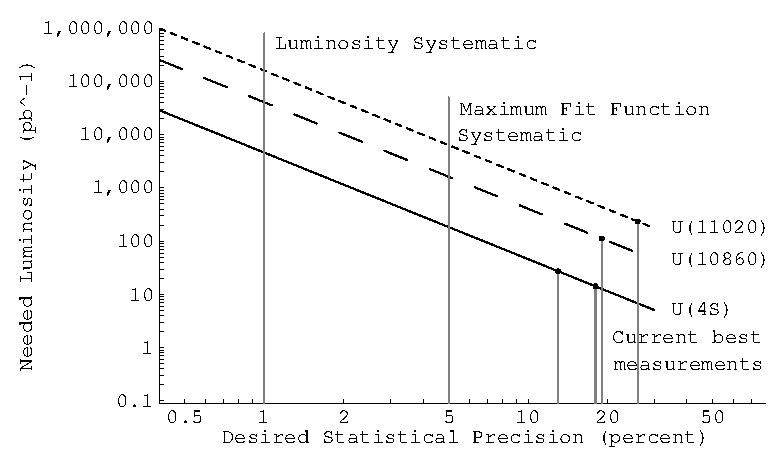
\epsfig{file=cleo_lumi_needed.eps, width=\textheight, angle=-90}
\end{center}

\end{slide*}

%%%%%%%%%%%%%%%%%%%%%%%%%%%%%%%%%%%%%%%%%%%%%%%%%%%%%%%%%%%%%%%%%%%%%%%%%%%

\end{document}

% %%%%%%%%%%%%%%%%%%%%%%%%%%%%%%%%%%%%%%%%%%%%%%%%%%%%%%%%%%%%%%%%%%%%%%%%%%%

% \begin{slide*}

% \slideframe{}
% \slideframe*[\dkblue]{Oval}
% \huge
% \heading{}

% \begin{minipage}[t]{\linewidth}

% \end{minipage}

% \end{slide*}


